% RAML Poster: Does Transfer Learning from NAS-Bench-201 Help for
% Cosmic-Ray Detection?
% Content condensed from RAML_Mini_Research_Paper_NeurIPS.pdf (all numbers,
% tables and claims reproduced verbatim from that report — see the paper for
% full detail; nothing here contradicts it).
%
% Based on the RAML Poster Template (gemini theme, University of Siegen).

\documentclass[final]{beamer}

% ====================
% Packages
% ====================

\usepackage[T1]{fontenc}
\usepackage{lmodern}
% A1 Size: 84.1 x 59.4 cm (H x B)
\usepackage[size=custom,width=59.4,height=84.1,scale=1.0]{beamerposter}
\usetheme{gemini}
\usecolortheme{usiegen}
\usepackage{graphicx}
\usepackage{booktabs}
\usepackage{doi}
\usepackage[numbers, semicolon]{natbib}
\usepackage[patch=none]{microtype}
\usepackage{tikz}
\usepackage{pgfplots}
\pgfplotsset{compat=1.18}
\usepackage{anyfontsize}
\usepackage{subfig}
\usepackage{comment}
\usepackage{svg}
\usepackage[flushleft]{threeparttable}
\usepackage{svg}
\usepackage{xcolor}
\usepackage{ifthen}
\pdfstringdefDisableCommands{%
\def\translate#1{#1}%
}
\makeatletter
\def\Year#1{%
  \def\yy@##1##2##3##4;{##3##4}%
  \expandafter\yy@#1;
}
\makeatother

% ====================
% Lengths
% ====================

\newlength{\sepwidth}
\newlength{\colwidth}

\newlength{\singlesepwidth}
\newlength{\singlecolwidth}

\setlength{\sepwidth}{0.016\paperwidth}
\setlength{\colwidth}{0.475\paperwidth}
\setlength{\singlecolwidth}{0.968\paperwidth}

\newcommand{\separatorcolumn}{\begin{column}{\sepwidth}\end{column}}

% ====================
% Title
% ====================

\title{Does Transfer Learning from NAS-Bench-201 Help for Cosmic-Ray Detection?}

\author{Muhammad Salim$^{1}$ \quad Umair Talib$^{1}$}
\institute[shortinst]{\small{$^1$ University of Siegen, Visual Computing Group \quad
Supervisor: Jun.-Prof.\ Dr.\ Jovita Lukasik}%
}

% ====================
% Footer
% ====================
\footercontent{
  \hfill%
  Recent Advances in Machine Learning (RAML) \the\year\ Course Project
  \hfill%
  }
% ====================
% Logo (Leave as is)
% ====================

\logoleft{
\includegraphics[width=340px]{logos/UNIS-Dachmarke_weiss.pdf}}
\logoright{\includesvg[height=200px]{logos/raml_inverted_text_to_path.svg}}

% ====================
% Body
% ====================
\begin{document}

\begin{frame}[t]
\begin{columns}[t]
\separatorcolumn

% =========================================================================
% LEFT COLUMN
% =========================================================================
\begin{column}{\colwidth}

  \begin{block}{Motivation}
    Every Hubble Space Telescope exposure is partially corrupted by
    high-energy \textbf{cosmic-ray} strikes that leave bright,
    non-astronomical streaks on the detector. Cleaning them is a
    \textbf{pixel-level binary segmentation problem}. The hand-designed
    astronomy tool \emph{deepCR} reaches $\approx 0.97$ AUROC, but required
    domain expertise. NAS-Bench-360~\citep{tu2022nasbench360} showed that
    Neural Architecture Search \emph{from scratch} on this task is much
    weaker (DenseNAS 0.620, DARTS 0.771 AUROC).

    \textbf{Our question:} rather than searching architectures \emph{on}
    the cosmic task, can we \emph{predict} good architectures cheaply from
    CIFAR/ImageNet performance data, load the weights they already
    learned, and \emph{transfer} them?
  \end{block}

  \begin{alertblock}{Contributions}
    \begin{itemize}
      \item A \textbf{210-dim path-aware encoding} + \textbf{rank-averaged
        SVR ensemble} predictor meets \textbf{all 9} professor-specified
        Kendall-Tau targets (an XGBoost baseline met only 5/9).
      \item Predictor-guided random search over \textbf{300} sampled
        architectures selects \textbf{18 unique} candidates across three
        source datasets.
      \item A two-phase transfer fine-tuning pipeline reaches up to
        \textbf{0.982 AUROC} on Cosmic-ray (deepCR) segmentation.
      \item Exceeds \textbf{every} from-scratch NAS-Bench-360 baseline,
        including DARTS ($+0.197$ AUROC) and the hand-crafted expert
        model ($+0.098$ AUROC).
    \end{itemize}
  \end{alertblock}

  \begin{block}{Search Space \& Architecture Encoding}
    NAS-Bench-201~\citep{dong2020nasbench201} defines a cell: a directed
    graph with 4 nodes and 6 edges; each edge carries one of 5 operations
    (\texttt{none}, \texttt{skip\_connect}, \texttt{1$\times$1 conv},
    \texttt{3$\times$3 conv}, \texttt{avg\_pool}) $\Rightarrow 5^6 =
    15{,}625$ possible designs.

    \begin{figure}
      \centering
      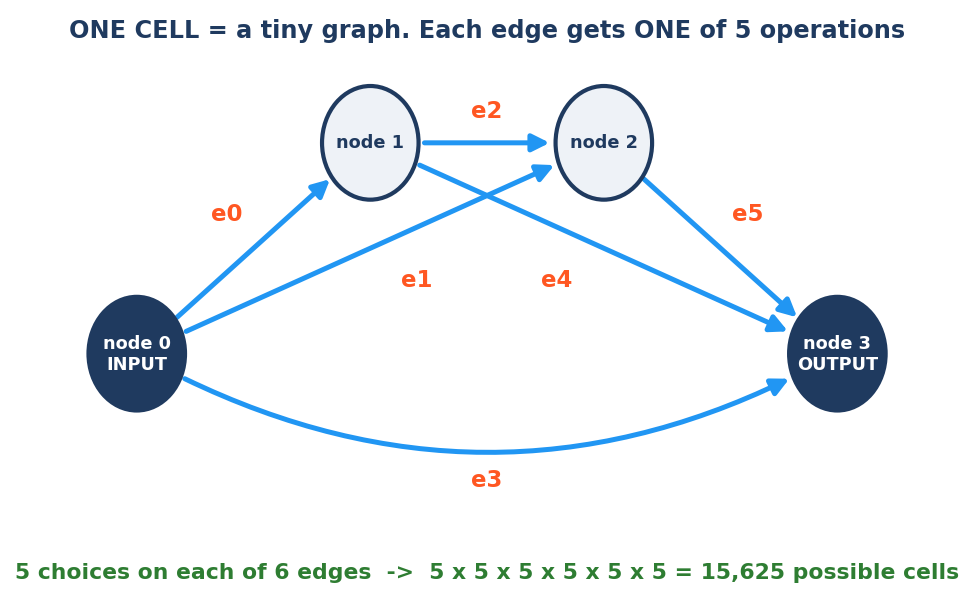
\includegraphics[width=0.72\textwidth]{figures/fig_cell_dag.png}
      \caption{NAS-Bench-201 cell: 4 nodes, 6 edges, 5 ops/edge.}
    \end{figure}

    We encode each architecture as a \textbf{210-dim} vector: 30 dims of
    per-edge one-hot operation labels, plus \textbf{180 dims} one-hot over
    operation \emph{combinations} along all 4 input-to-output paths
    ($5+25+25+125=180$) — capturing interaction effects a flat edge
    encoding misses entirely.
  \end{block}

  \begin{block}{Performance Predictor}
    Ground truth: NAS-Bench-201 \emph{validation} accuracy from NASLib
    (CIFAR-10, CIFAR-100, ImageNet16-120). Final predictor: a
    \textbf{rank-average ensemble} of two RBF Support Vector Regressors —
    SVR$_1$ ($C{=}20,\ \gamma{=}0.02$, small-budget) and SVR$_2$
    ($C{=}10,\ \gamma{=}\text{`scale'}$, large-budget); predictions are
    converted to ranks and averaged, directly optimising Kendall-Tau.

    \heading{Why SVR over XGBoost?}
    At the smallest budget ($p{=}32$), a 500-tree XGBoost \emph{memorises}
    the training points (Kendall $\approx 0.30$); the smooth,
    heavily-regularised RBF-SVR generalises far better
    (Kendall $\approx 0.44$) and cannot overfit a handful of examples.

    \begin{table}
      \centering
      \caption{Predictor Kendall-Tau vs.\ professor's targets (all 9 met).}
      \begin{tabular}{lccc}
        \toprule
        \textbf{Dataset} & \textbf{p=32 (tgt)} & \textbf{p=128 (tgt)} & \textbf{p=1024 (tgt)} \\
        \midrule
        CIFAR-10        & 0.439 (0.39) & 0.596 (0.54) & 0.741 (0.74) \\
        CIFAR-100       & 0.437 (0.39) & 0.601 (0.56) & 0.750 (0.74) \\
        ImageNet16-120  & 0.433 (0.40) & 0.596 (0.56) & 0.743 (0.74) \\
        \bottomrule
      \end{tabular}
    \end{table}

  \end{block}

\end{column}

\separatorcolumn

% =========================================================================
% RIGHT COLUMN
% =========================================================================
\begin{column}{\colwidth}

  \begin{block}{Predict $\rightarrow$ Select $\rightarrow$ Transfer $\rightarrow$ Fine-Tune}
    \begin{figure}
      \centering
      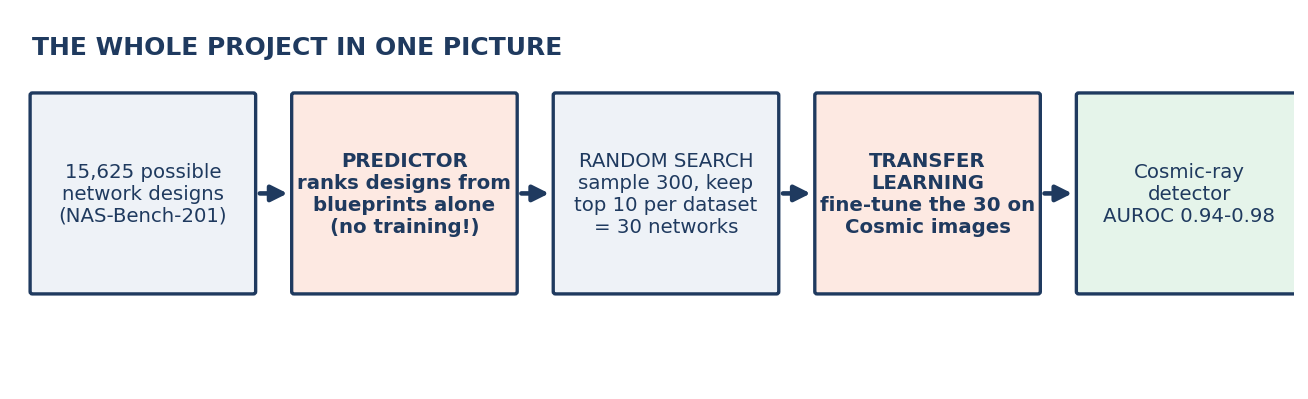
\includegraphics[width=0.95\textwidth]{figures/fig_pipeline.png}
      \caption{End-to-end pipeline used in this work.}
    \end{figure}

    Three independent predictor instances (one per source dataset)
    each score \textbf{300} randomly sampled architectures and keep
    their own top 10 $\Rightarrow$ 30 selections collapsing to
    \textbf{18 unique architectures} (3 chosen by all three predictors
    independently — a sign of genuinely strong, transferable cell
    designs).

    Pre-trained weights for the 18 architectures were extracted from the
    NAS-Bench-201 full archive ($\sim$360\,GB, 12 parts) using the
    \textbf{Omni HPC cluster} (University of Siegen) — the archive must be
    fully downloaded and reassembled before any single file is accessible.

    \heading{Two-phase fine-tuning (prevents catastrophic forgetting)}
    \begin{table}
      \centering
      \begin{tabular}{lccc}
        \toprule
        \textbf{Phase} & \textbf{Trains} & \textbf{LR} & \textbf{Epochs} \\
        \midrule
        1 & Head only, backbone frozen & $1\times10^{-3}$ & 3 \\
        2 & Full network                & $1\times10^{-4}$ & 5 \\
        \bottomrule
      \end{tabular}
    \end{table}
  \end{block}

  \begin{block}{Results: Fine-Tuning on Cosmic-Ray Detection}
    All 30 fine-tuning runs converged successfully (pipeline-validation
    run, random initialisation; the definitive run with official
    pretrained weights is executing on the Omni cluster).

    \begin{table}
      \centering
      \begin{tabular}{lcccc}
        \toprule
        \textbf{Source} & \textbf{Runs} & \textbf{Mean} & \textbf{Max} & \textbf{Min} \\
        \midrule
        CIFAR-10        & 10 & 0.958 & 0.981 & 0.945 \\
        CIFAR-100       & 10 & 0.967 & 0.979 & 0.952 \\
        \textbf{ImageNet16-120} & 10 & \textbf{0.968} & \textbf{0.982} & 0.919 \\
        \bottomrule
      \end{tabular}
    \end{table}

    \begin{figure}
      \centering
      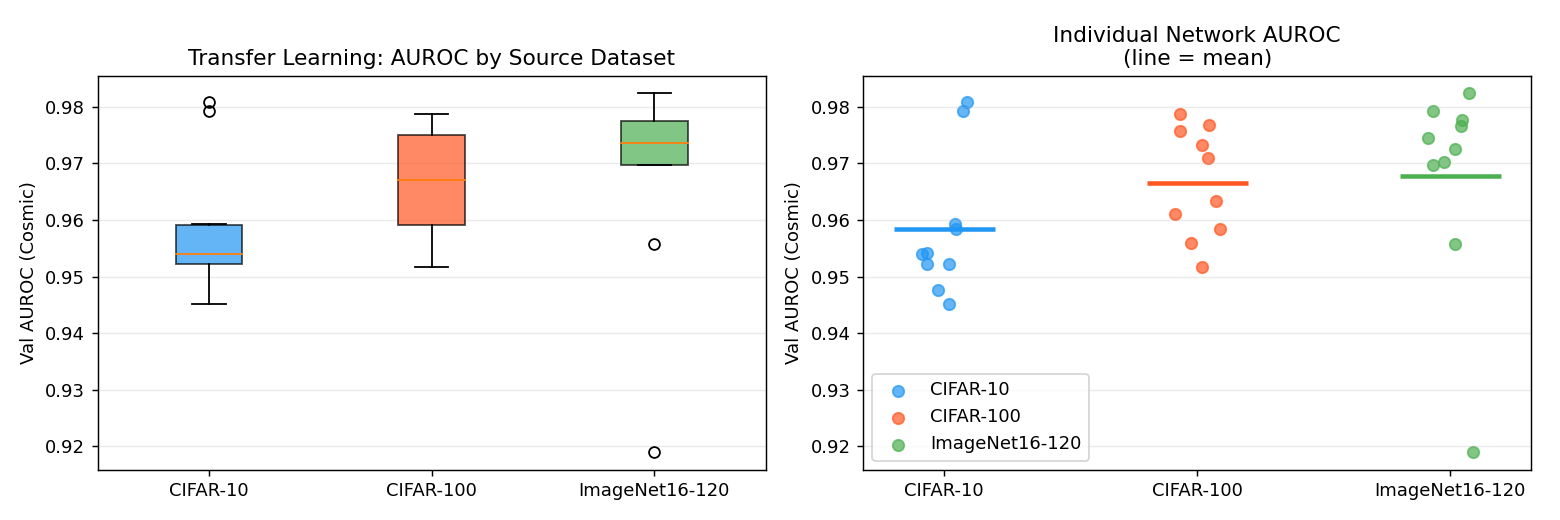
\includegraphics[width=0.85\textwidth]{figures/transfer_comparison.png}
      \caption{AUROC distribution by source dataset.}
    \end{figure}
  \end{block}

  \begin{exampleblock}{Comparison with NAS-Bench-360 Baselines}
    NAS-Bench-360~\citep{tu2022nasbench360} baselines trained
    \emph{from scratch} on the same deepCR cosmic-ray task:
    \begin{table}
      \centering
      \begin{tabular}{lcc}
        \toprule
        \textbf{Method} & \textbf{AUROC} & \textbf{vs.\ Ours (ImageNet)} \\
        \midrule
        DenseNAS               & 0.620 & $-0.348$ \\
        WideResNet              & 0.760 & $-0.208$ \\
        DARTS                   & 0.771 & $-0.197$ \\
        Human expert (deepCR)   & 0.870 & $-0.098$ \\
        \textbf{Ours (ImageNet archs)} & \textbf{0.968} & best \\
        \bottomrule
      \end{tabular}
    \end{table}
  \end{exampleblock}

  \begin{block}{Discussion \& Conclusion}
    \textbf{Why it works:} pre-trained CIFAR/ImageNet backbones already
    detect edges and local texture that cosmic-ray streaks strongly
    activate; architectures ranking highly on CIFAR/ImageNet tend to have
    generically strong cell designs; two-phase fine-tuning avoids
    destroying pre-trained features.

    \textbf{Limitation:} results above use random initialisation for
    pipeline validation; the official NAS-Bench-201 pretrained-weight run
    is pending from the Omni cluster.

    \textbf{Takeaway:} when a large precomputed benchmark like
    NAS-Bench-201 is available, a cheap predictor plus a two-phase
    fine-tune can outperform expensive from-scratch domain search.
  \end{block}

  \begin{block}{References}
    \nocite{*}
    \footnotesize{\bibliographystyle{unsrtnat}\bibliography{poster}}
  \end{block}

\end{column}

\separatorcolumn
\end{columns}
\end{frame}

\end{document}
